%%%%%%%%%%%%%%%%%%%%%%%%
%
% $Author: Sadegh Naderi $
% $Datum: 2024-02-10  $
% $Pfad: ML23-01-Keyword-Spotting-with-an-Arduino-Nano-33-BLE-Sense\Poster\KeywordSpottingPoster.tex $
% $Version: 1.0 $
% $Reviewed by: Sadegh Nader $
% $Review Date: 2024-02-12 $
%
%%%%%%%%%%%%%%%%%%%%%%%%

\documentclass[25pt,a0paper, portrait]{tikzposter}
\usepackage[utf8]{inputenc}
\usepackage{xcolor}
\usepackage{graphicx,mwe}
\usepackage{filecontents}
\usepackage{lipsum}
\usepackage{tikz}
\usepackage{multicol}
\usepackage{adjustbox}
\usepackage{blindtext}
\usepackage{comment}


\makeatletter
\def\TP@titlegraphictotitledistance{-6cm}
\settitle{ \centering \vbox{
		\@titlegraphic \\ [\TP@titlegraphictotitledistance] 
		\centering
		\color{titlefgcolor} 
		{\bfseries \Huge \sc \@title \par}
		\vspace*{1em}
		{\huge \@author \par}
}}
\makeatother

\setlength{\columnsep}{2cm}

\title{Keyword Spotting}
\author{Sadegh Naderi, Malik Ghansletwala, Achal Shakywar}
\titlegraphic{
\includegraphics[height=6.5cm]{images/logoHSEmdenLeer}
	\hfill
	
\includegraphics[height=6.5cm]{images/logoBIDA}
}


\usetheme{Desert}

\begin{document}
	
	\maketitle
	
	\begin{columns} 
		
		\column{0.4}
		{
			\colorlet{blocktitlebgcolor}{blue}
			\block{Problem Description}
			{
				
				This project addresses concerns around data privacy and connectivity by bringing voice recognition to the edge. Utilizing TinyML in embedded machine learning, the project showcases the fusion of machine learning and embedded systems, enabling the board Arduino Nano 33 BLE Sense to recognize keywords directly. This reduces the reliance on cloud processing, enhancing user privacy and creating offline-capable voice-activated solutions. The compact and resource-efficient nature of the board Arduino Nano 33 BLE Sense exemplifies the potential for privacy-aware interactions in various domains, from home automation to assistive technologies.
				
				
				
			}
		}
		
		\colorlet{blocktitlebgcolor}{blue}
		\block{Challenges}
		{
			
			\begin{itemize}
				\item \textbf{Data Collection:} Gathering a diverse and representative dataset for training the machine learning model can be challenging \cite{Nabaz:2023}.
				
				\item \textbf{Hardware and software heterogeneity:} Variability in hardware and software infrastructure complicates the adoption of consistent learning and deployment strategies for TinyML systems \cite{Ray:2022}.
				
				\item \textbf{Model Size:} Since the model will be deployed on a resource-constrained device, it needs to be small in size. Balancing model size with accuracy and performance is a significant challenge \cite{Abbas:2023}. Optimization and quantization of the model is required to ensure it works well within the device's limitations \cite{Ray:2022}.
				\item\textbf{Noise and Variability Handling:} Developing a robust keyword spotting system that accommodates speech variations, accents, and environmental noise is challenging for practical applications \cite{Warden:2018}.
			\end{itemize}
			
		}
		
		
		
		\colorlet{blocktitlebgcolor}{blue}
		\block{Solution}
		{
			\begin{itemize}
				\item The devised solution leverages a Convolutional Neural Network (CNN) architecture for keyword spotting on the board Arduino Nano 33 BLE Sense.
				\item The model takes spectrogram images as input, undergoing a series of transformations, including downsampling, normalization, convolutional operations, and max-pooling to extract relevant features.
				\item The final flattened output is converted into a 1D array.
				\item The model is saved and converted to TensorFlow Lite format, generating a C header file.
				\item The C header file is then integrated into the TensorFlow library within the Arduino IDE.
				\item The finalized model is uploaded onto the board Arduino Nano 33 BLE Sense.
			\end{itemize}
			
			
		}
		
		\colorlet{blocktitlebgcolor}{blue}
		\block{Data Transformation}
		{
			\begin{tikzfigure}
				
				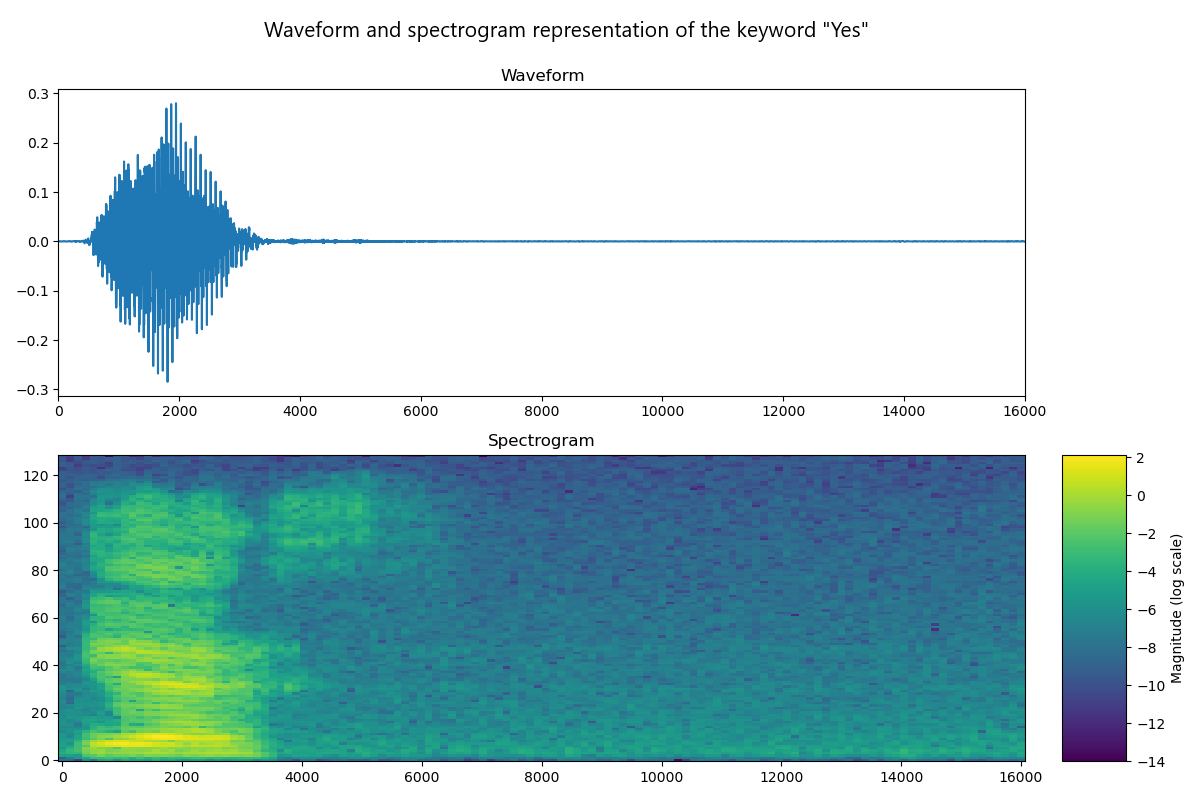
\includegraphics[width=\linewidth]{images/audioWaveSpectrogramYes}
				
			\end{tikzfigure}
			
		    To convert audio to a spectrogram, one-second audio snippets are analyzed in a loop, applying fast Fourier transform (FFT) to each 30-millisecond segment with a 20-millisecond overlap. This process produces a 2D array representing the entire audio sample. This 2D array, commonly known as a spectrogram, captures the intensity of different frequency components across time. The spectrogram is then fed to the CNN model.
		
		}
		
		
		\column{0.56}
		{
			\colorlet{blocktitlebgcolor}{blue}
			\block{Dataset}
			{
				The dataset prioritizes realistic audio capture by steering clear of studio-captured samples, ensuring the presence of background noise and utilizing phone or laptop microphones. The focus is on English language, incorporating various accents beyond American English, recorded from several individuals to ensure speaker independence. The dataset comprises one-second single words in WAV format, with a sample rate set to 16 KHz. It boasts a dataset size of 8.17 GB, and a selected data subset of 415 MB, all while maintaining open-source and anonymous attributes, avoiding the recording of personally identifiable information. Additionally, background noise files were included for training and testing the model's ability to differentiate between speech and non-speech audio. The primary emphasis of the dataset revolves around specific keywords, namely: "yes," "no," "up," "down," "stop," "go," "left," and "right." The keywords "yes" and "no" are chosen for the Board to take response to. The Board is programmed to respond to the keywords "yes" and "no."
			}

		}
		
		\colorlet{blocktitlebgcolor}{blue}
		\block{Model Evaluation Metrics}
		{
			\begin{itemize}
				\item \textbf{Accuracy}: This metric indicates the proportion of correctly classified instances out of the total number of instances. 
				
				\item \textbf{Loss}: The loss is a measure of how well the model is performing, with the goal of minimizing this value. It represents the error between the predicted outputs and the actual targets. 
			\end{itemize}
		}
		
		\colorlet{blocktitlebgcolor}{blue}
		\block{Results}
		{			
			The CNN model has reached a training accuracy of 89.39\% and a training loss of 0.32. The validation accuracy is 86\%, and the validation loss is 0.42. The accuracy of the model on test data is 85\%.
			
			There is room for improvement in terms of generalization, as indicated by the slightly higher validation loss and the training loss. Further tuning, regularization techniques, or adjustments to the model architecture may be considered to enhance overall performance on unseen data.
			
			\begin{tikzfigure}
				\begin{minipage}[b]{0.29\linewidth}
					\centering
					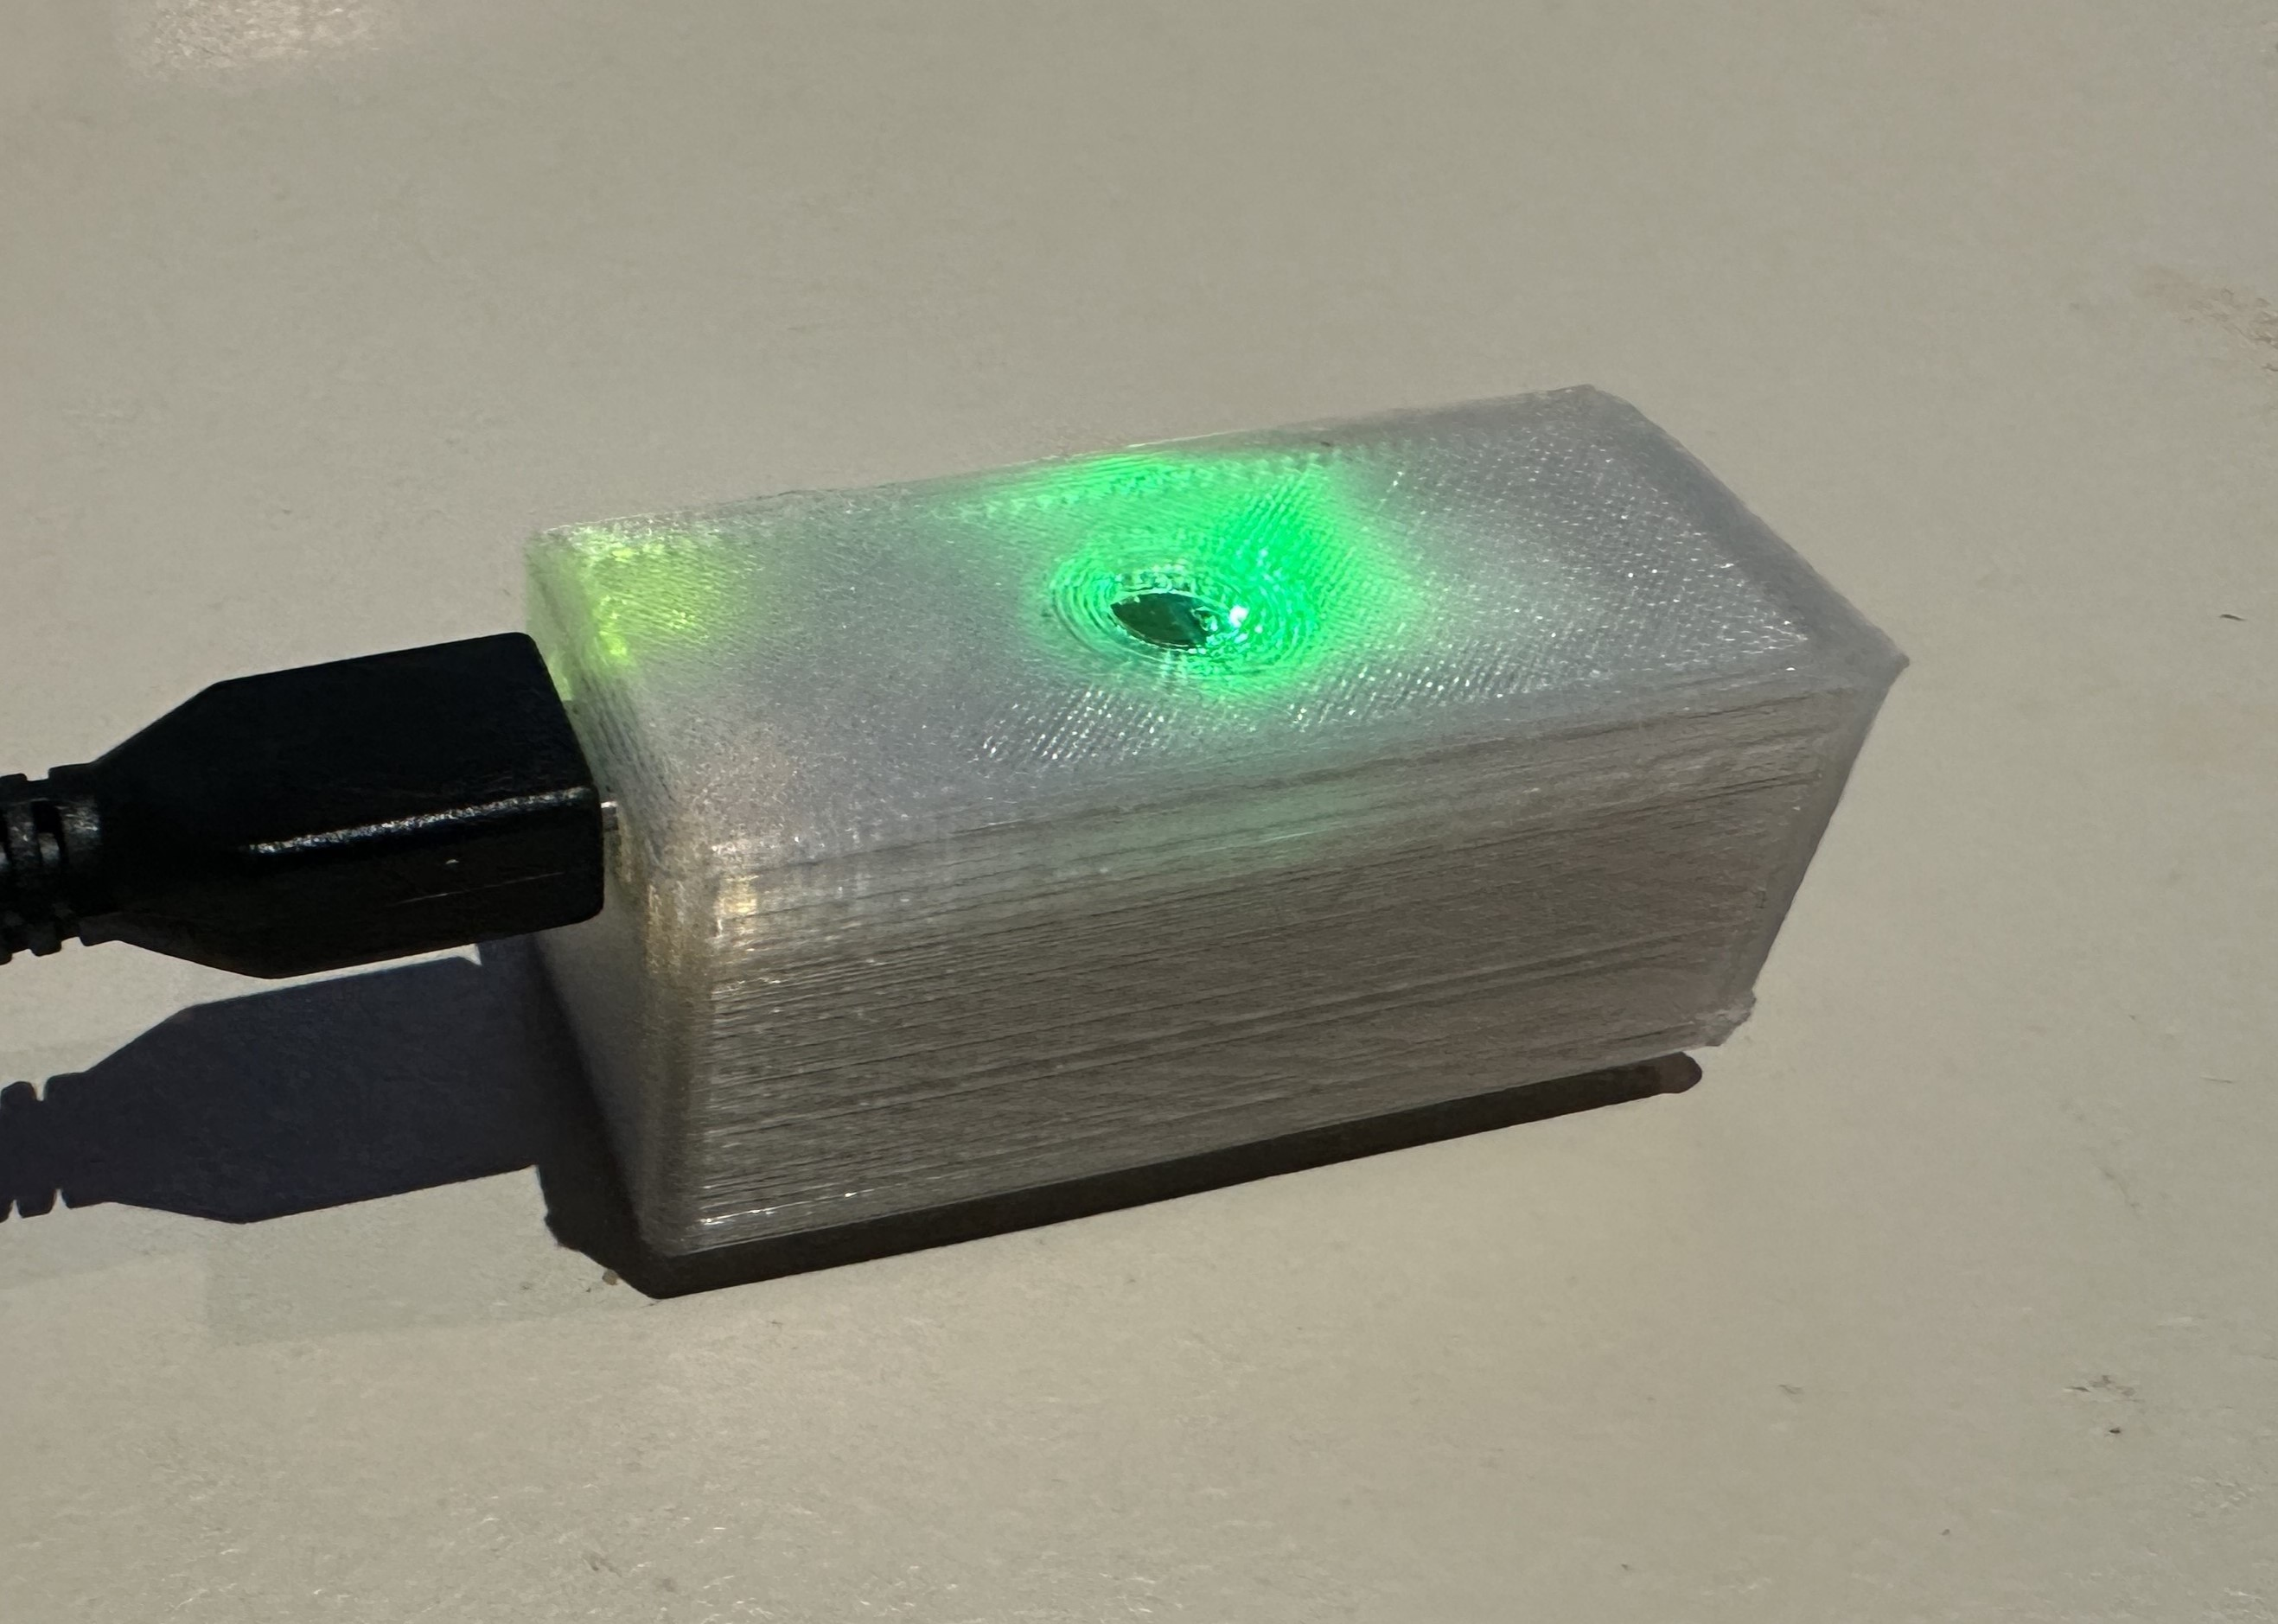
\includegraphics[width=\linewidth]{images/ArduinoGreen}
				\end{minipage}
				\hfill
				\begin{minipage}[b]{0.33\linewidth}
					\centering
					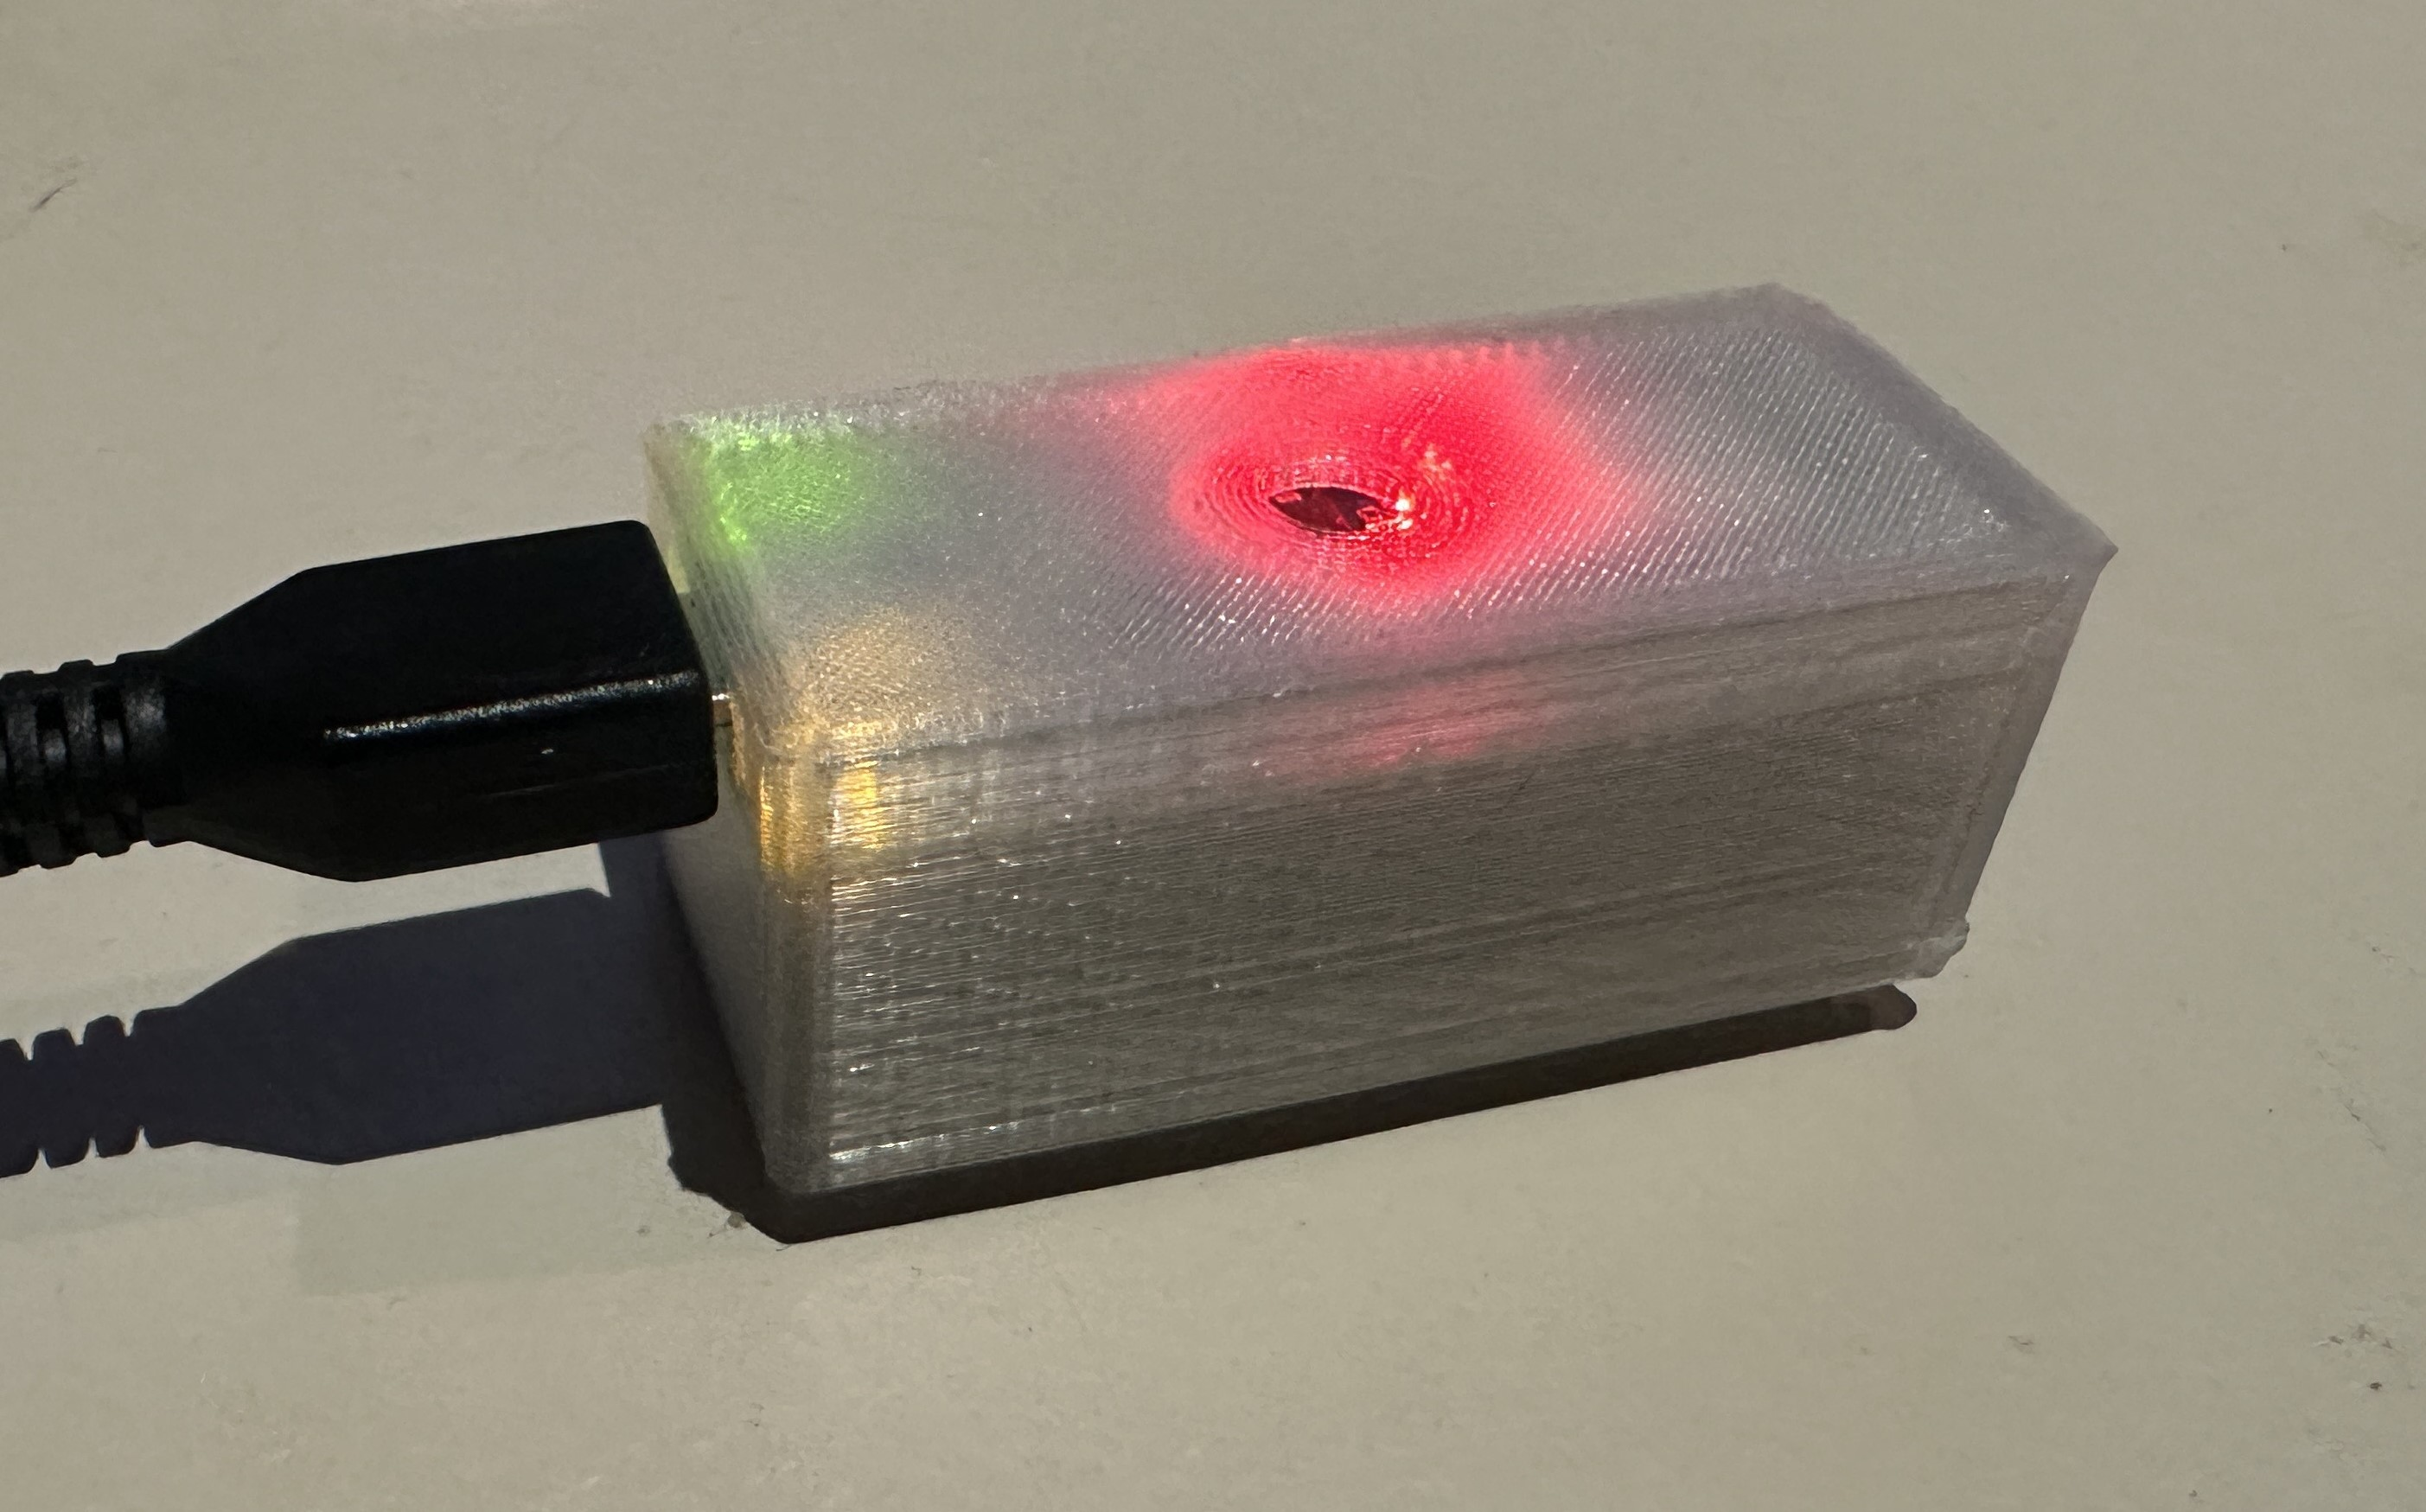
\includegraphics[width=\linewidth]{images/ArduinoRed}
				\end{minipage}
				\hfill
				\begin{minipage}[b]{0.3\linewidth}
					\centering
					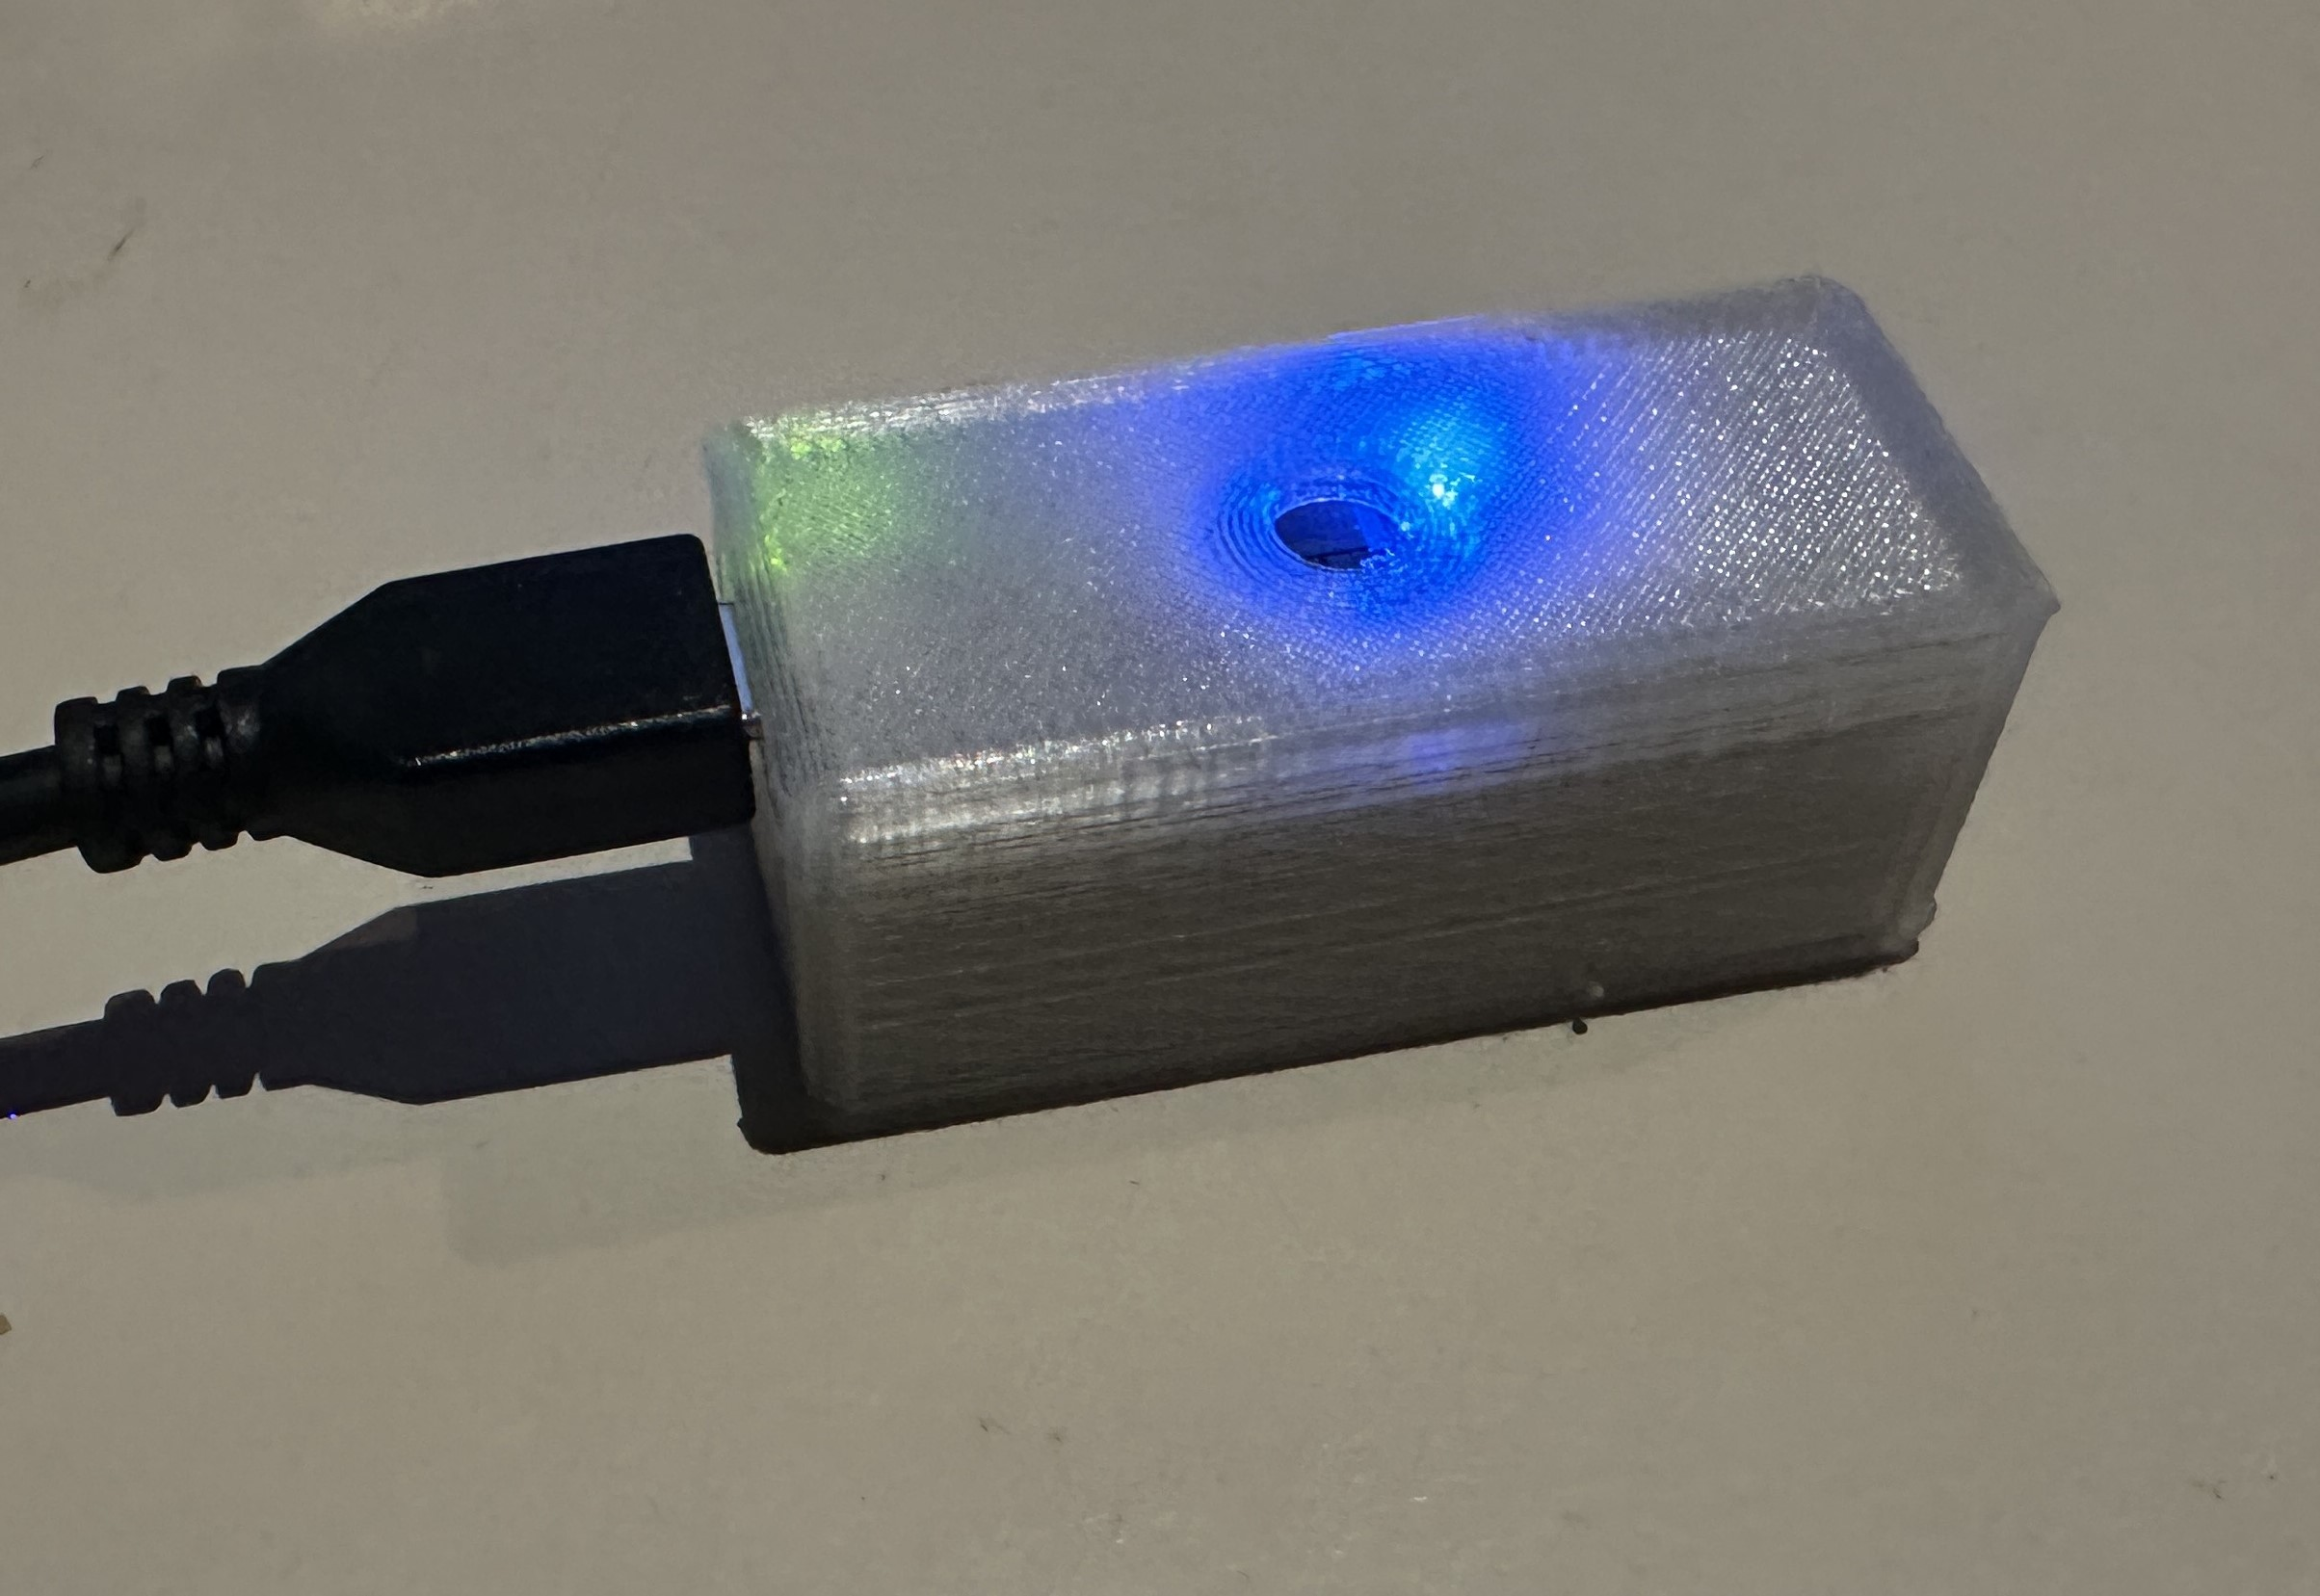
\includegraphics[width=\linewidth]{images/ArduinoBlue}
				\end{minipage}
			\end{tikzfigure}
			
			
			The board's LED responses:
			
			\begin{itemize}
				\item \textbf{Green:} Reesponse to the "yes" keyword.
				\item \textbf{Red:} Reesponse to the "No" keyword.
				\item \textbf{Blue:} Reesponse to an unknown keyword.
			\end{itemize}
			
			The board shows relatively accurate responses. To trigger a response, the speaker needs to utter the keyword within a 20cm range. Occasionally, the board may not register any response, and at times, it might mistakenly classify a "yes" or "no" keyword as an unfamiliar term, indicated by a blue LED. At times, the board may exhibit an unknown keyword response due to environmental noise.
			
		}
		
		\colorlet{blocktitlebgcolor}{blue}
		\block{Future Work}
		{
			\begin{itemize}
				\item \textbf{Model Optimization:} Investigate further optimization techniques to reduce the model size without compromising performance. Delve into the realm of quantization methods, and model compression techniques.
				
				\item \textbf{Improve model Robustness:} Explore techniques for improving the robustness of the model against variations in input, including different accents, speaking rates, and background noise. This may involve augmenting the training dataset with more diverse examples and incorporating robustness-enhancing strategies during model training.
				
				\item \textbf{Machine Learning Model Iterations:} Explore advanced machine learning models, beyond Convolutional Neural Networks, to enhance keyword recognition on resource-constrained devices. Use diverse model architectures, including recurrent neural networks, and transformer models.
				
			\end{itemize}
			
		}
		
		
		\colorlet{blocktitlebgcolor}{blue}
		\block{References}
		{			
			\small
			\bibliographystyle{plain}
			\bibliography{../Documents/MyLiterature.bib}
			
		}
		
		
	\end{columns}
	
\end{document}

